\documentclass{article}

\usepackage[utf8]{inputenc}
\usepackage{graphicx}

\graphicspath{ {images/} }

\usepackage[backend=biber]{biblatex}
\addbibresource{bibliography.bib}

\begin{document}
\title{Projeto Latex: Informática Teórica — IF689}
\author{Beatriz Férre}
\date{Dezembro 2021}
\maketitle

\begin{abstract}
Apresentação ao objeto de estudo e aplicações da disciplina de Informática Teórica, oferecida pelo Centro de Informática da UFPE.
\end{abstract}
\section{Introdução}


Informática Teórica é uma disciplina voltada para as \textit{propriedades matemáticas fundamentais} do hardware, do software, e das aplicações de computadores. Seu estudo visa compreender os limites da computação, os custos de cada processo na memória e os diferentes modelos computacionais passíveis de uso. Suas áreas centrais são: \textbf{autômatos, computabilidade e complexidade.} Visando sempre as aplicações à computação, bases matemáticas essenciais para a área de T.I são lançadas com o conhecimento teórico adquirido nessa cadeira. A partir da compreensão desses paradigmas, é possível criar algoritmos, modelos e sistemas mais seguros e completos, ou até renovar o modo como eles são pensados.
\cite{introduction}

\section{Relevância}

O estudo da Informática Teórica é útil para a \textbf{compreensão lateral} da área de ciência da computação, visto que os modelos nela analisados são parte integral da história e do “inconsciente coletivo” do campo. A computação é fortemente baseada, explícita ou implicitamente, nos \textit{paradigmas teóricos da informática}, de tal forma que o contato com eles desde cedo garante ao estudante e ao profissional um olhar mais versado com relação a métodos de resolução de problemas.

Além disso, projetos e experimentos que revolucionaram a computação só foram possíveis graças ao extenso estudo de acadêmicos quanto ao que pode ou não ser computado, quanto de memória é gasto em um processo, o quão rápido ele ocorre, dentre outros aspectos abordados nessa disciplina. A computação só é possível graças aos teóricos que buscaram e ainda buscam soluções mais elegantes e matematicamente sólidas para os problemas computacionais.
\cite{elements}
 
\section{Relação com outras disciplinas}
Sendo fundamentada em \textit{princípios matemáticos}, conceitos de várias disciplinas teóricas e matemáticas são basilares para o entendimento da Informática Teórica. 

\begin{figure}[ht]
    \centering
    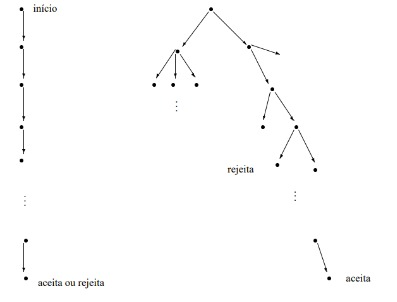
\includegraphics[width=0.85\textwidth]{grafos}
    \caption{ representação em grafos (vistos em matemática discreta) no estudo de determinismo computacional}
    \label{fig:exemplo1}
\end{figure}

Por exemplo, assuntos abordados na disciplina de \textbf{Matemática Discreta} como \textit{conjuntos, sequências e grafos} (figura \ref{fig:exemplo1}) são explorados por um viés computacional, aplicando o que é estudado no desenvolvimento de códigos.

\begin{figure}[ht]
    \centering
    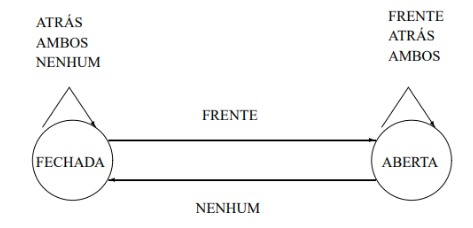
\includegraphics[width=0.85\textwidth]{logica}
    \caption{ aplicação do conceito de estados booleanos na transição de \emph{Turing Machines}}
    \label{fig:exemplo2}
\end{figure}

Em outro exemplo, dado pela figura \ref{fig:exemplo2}, a Informática Teórica também se vale de \textit{conceitos de Lógica} como operadores booleanos e provas lógicas no estudo da \textit{complexidade de máquinas} e \textit{computabilidade} de algoritmos. 
\cite{complexity}

De forma geral, a visão teórica de informática está presente de forma latente em toda disciplina que se propõe a lançar as \textbf{bases conceituais necessárias} para o \textit{approach} correto de desenvolvimento. Consequentemente, disciplinas práticas como \textbf{Introdução à Programação, Algoritmos e Engenharia de Softwares e Sistemas} são mais bem aproveitadas quando se tem a bagagem que a Informática Teórica oferece. 

\begin{figure}[ht]
    \centering
    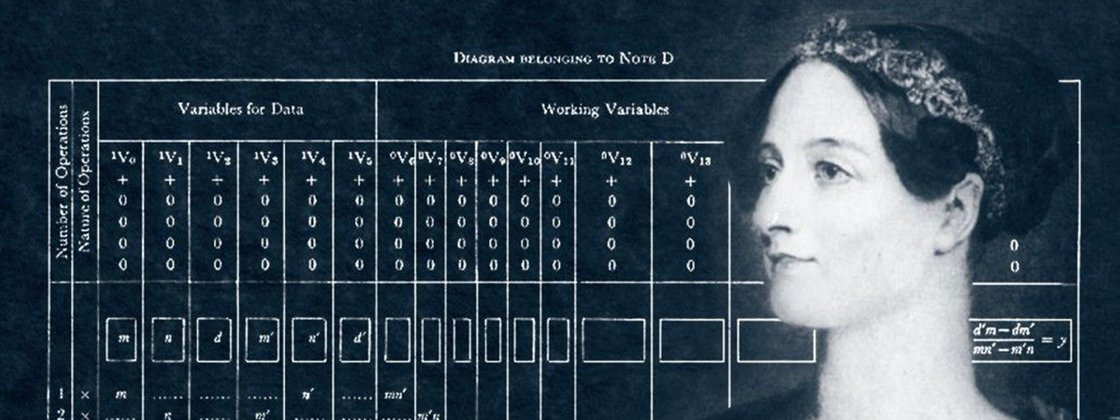
\includegraphics[width=0.75\textwidth]{adalov}
    \caption{Ada Lovelace, considerada a primeira programadora da história}
    \label{fig:ada}
\end{figure}

 Para exemplificar essa interligação entre a teoria e as disciplinas práticas, a programação de computadores como a entendemos ocorreu somente anos depois de Ada Lovelace (figura \ref{fig:ada}) escrever a teoria algorítmica por trás de uma máquina de computar conhecida como Máquina Analítica.\cite{adalovelace}

\printbibliography[
heading=bibintoc,
title={Referências}
]
\end{document}
